\section{\Cyclus}
\subsection{Ethos of \Cyclus}
% ---------------------------------------------- %
% Cyclus
\begin{frame}{History and Goals of \Cyclus}
\begin{itemize}
    \item Successor to Global Evaluation of Nuclear Infrastructure Utilization Scenarios (GENIUS) tools
\end{itemize}

\alert{Goal: Flexibility}

\begin{itemize}
    \item Model innovative/unconventional technologies
    \item Minimal inherent technology assumptions
\end{itemize}

\alert{Goal: Modeling}

\begin{itemize}
    \item Discrete facilities with discrete material tracking
    \item Optimization and sensitivity analysis
\end{itemize}

\alert{Goal: Software}


\begin{itemize}
    \item Low barrier to adoption with rapid payback\footnote{The goal we're probably furthest from at this moment}
    \item Commonly and freely available software infrastructure, can run on all operating systems
\end{itemize}
\end{frame}
% ---------------------------------------------- %



\subsection{Agent-based modeling}
% ---------------------------------------------- %
% Cyclus
\begin{frame}{\Cyclus Overview\cite{huff_fundamental_2016}}

\begin{columns}
\column{0.5\textwidth}
\begin{figure}
    \centering
    
\includegraphics[width=0.4\textwidth]{images/logo2.png}
    \label{fig:my_label}
\end{figure}
\begin{itemize}
    \item Open source modular fuel cycle simulator
    \item Market-based exchange of resources (commodities)
    \item Discrete facilities (even when identical)
    \item Discrete material tracking at the nuclide level
    \item Time-dependent
    \item Parallelizable
\end{itemize}
\column{0.5\textwidth}
\begin{figure}
    \centering
    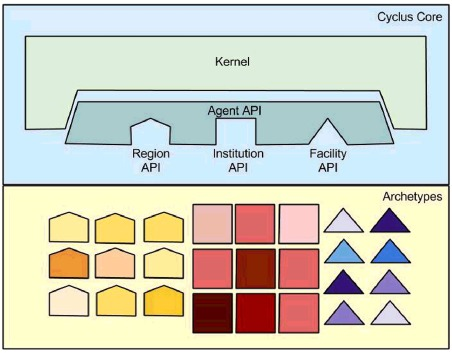
\includegraphics[width=0.9\textwidth]{images/cyclus_region_inst_facility.jpg}
    \caption{From \textit{Fundamental concepts in the Cyclus nuclear fuel cycle simulation framework} by Huff \textit{et al.}\cite{huff_fundamental_2016}}
    \label{fig:Cyclus_setup}
\end{figure}
\end{columns}

\end{frame}
% ---------------------------------------------- %


% ---------------------------------------------- %
\begin{frame}{Agent-based model}
\begin{columns}
\column{0.45\textwidth}
\begin{itemize}
    \item \Cyclus coordinates and tracks the \textbf{deployment of facilities} and \textbf{movement of materials between facilities}
    \item Facility models are "plug and play" through the API
    \item Allow for easy switch between lower and higher fidelity
    \item Similar to MOOSE framework collaboration
\end{itemize}
\column{0.5\textwidth}
\begin{figure}
    \centering
    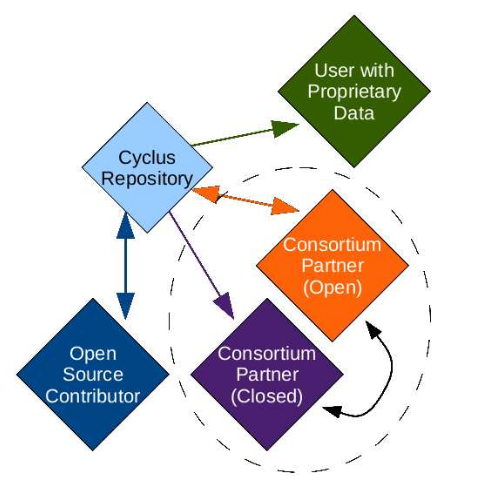
\includegraphics[width=0.85\textwidth]{images/Cyclus_ecosystem.png}
    \caption{\Cyclus architecture encourages open collaboration while allowing closed development and users with sensitive information, image from \cite{huff_fundamental_2016}}
    \label{fig:cyclus_ecosystem}
\end{figure}
\end{columns}
\end{frame}
% ---------------------------------------------- %



% ---------------------------------------------- %
\begin{frame}{\Cyclus facility models}
\begin{columns}
\column{0.45\textwidth}
\begin{itemize}
    %\item \Cyclus Kernel only requires the ability to place and respond to bids (trade)
    \item \Cycamore includes simple models of common fuel cycle facilities
    \item Developers have contributed higher fidelity models such as 
    \begin{itemize}
        \item cyborg (Univ. of Tennessee)
        \item mbmore (Univ. of Wisconsin)
    \end{itemize}
    \item Anyone can develop an archetype
    \begin{itemize}
        \item Open and closed contributors, models (archetypes), and users
    \end{itemize}
\end{itemize}
\column{0.5\textwidth}
\begin{figure}
    \centering
    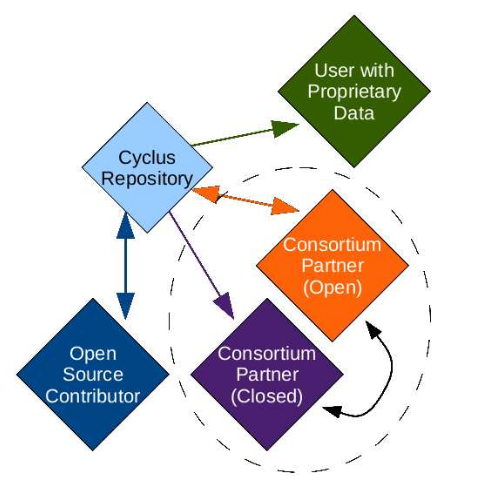
\includegraphics[width=0.85\textwidth]{images/Cyclus_ecosystem.png}
    \caption{\Cyclus architecture encourages open collaboration while allowing closed development and users with sensitive information, image from \cite{huff_fundamental_2016}}
    \label{fig:cyclus_ecosystem}
\end{figure}
\end{columns}
\end{frame}
% ---------------------------------------------- %


\subsection{Market Exchange of Commodities}
% ---------------------------------------------- %
\begin{frame}{Dynamic Resource Exchange}
\begin{itemize}
    \item At every timestep, \Cyclus gathers information about commodity requests
    \begin{itemize}
        \item Quantity
        \item Quality (isotopics)
        \item Can be XOR, such as MOX or UOX
    \end{itemize}
    \item \Cyclus then gathers bids and solves the flow graph
    \item Materials are transferred and the simulation moves forward to the next timestep
    \item Market-based exchange of resources (commodities)
    \begin{itemize}
        \item Nuclear materials
        \item Knowledge, design information, experts
        \item Economic units, money
    \end{itemize}
\end{itemize}
\end{frame}
% ---------------------------------------------- %

% ---------------------------------------------- %
\begin{frame}{Regions and Institutions}
    \begin{itemize}
        \item Reflects the geopolitical realities of nuclear facilities 
        \item Hierarchy is Region, Institution, Facility
        \item Region: State, could also be a geographical region smaller (e.g. the Midwest), or larger (e.g. Scandinavia) than a State 
        \item Institution: utility or government
        \item Institutions deploy facilities
        \item Flow can be prioritized within institution/region
        \item Institutions can reject material outside desired characteristics (e.g. above 5\% enriched) from other institutions
        \item Can be ignored (set to Null) if not relevant for a given simulation
    \end{itemize}
\end{frame}
% ---------------------------------------------- %


\subsection{\Cyclus Community}
% ---------------------------------------------- %
\begin{frame}{\Cyclus Community}
    \begin{columns}
    \column{0.9\textwidth}
    \begin{figure}
        \centering
        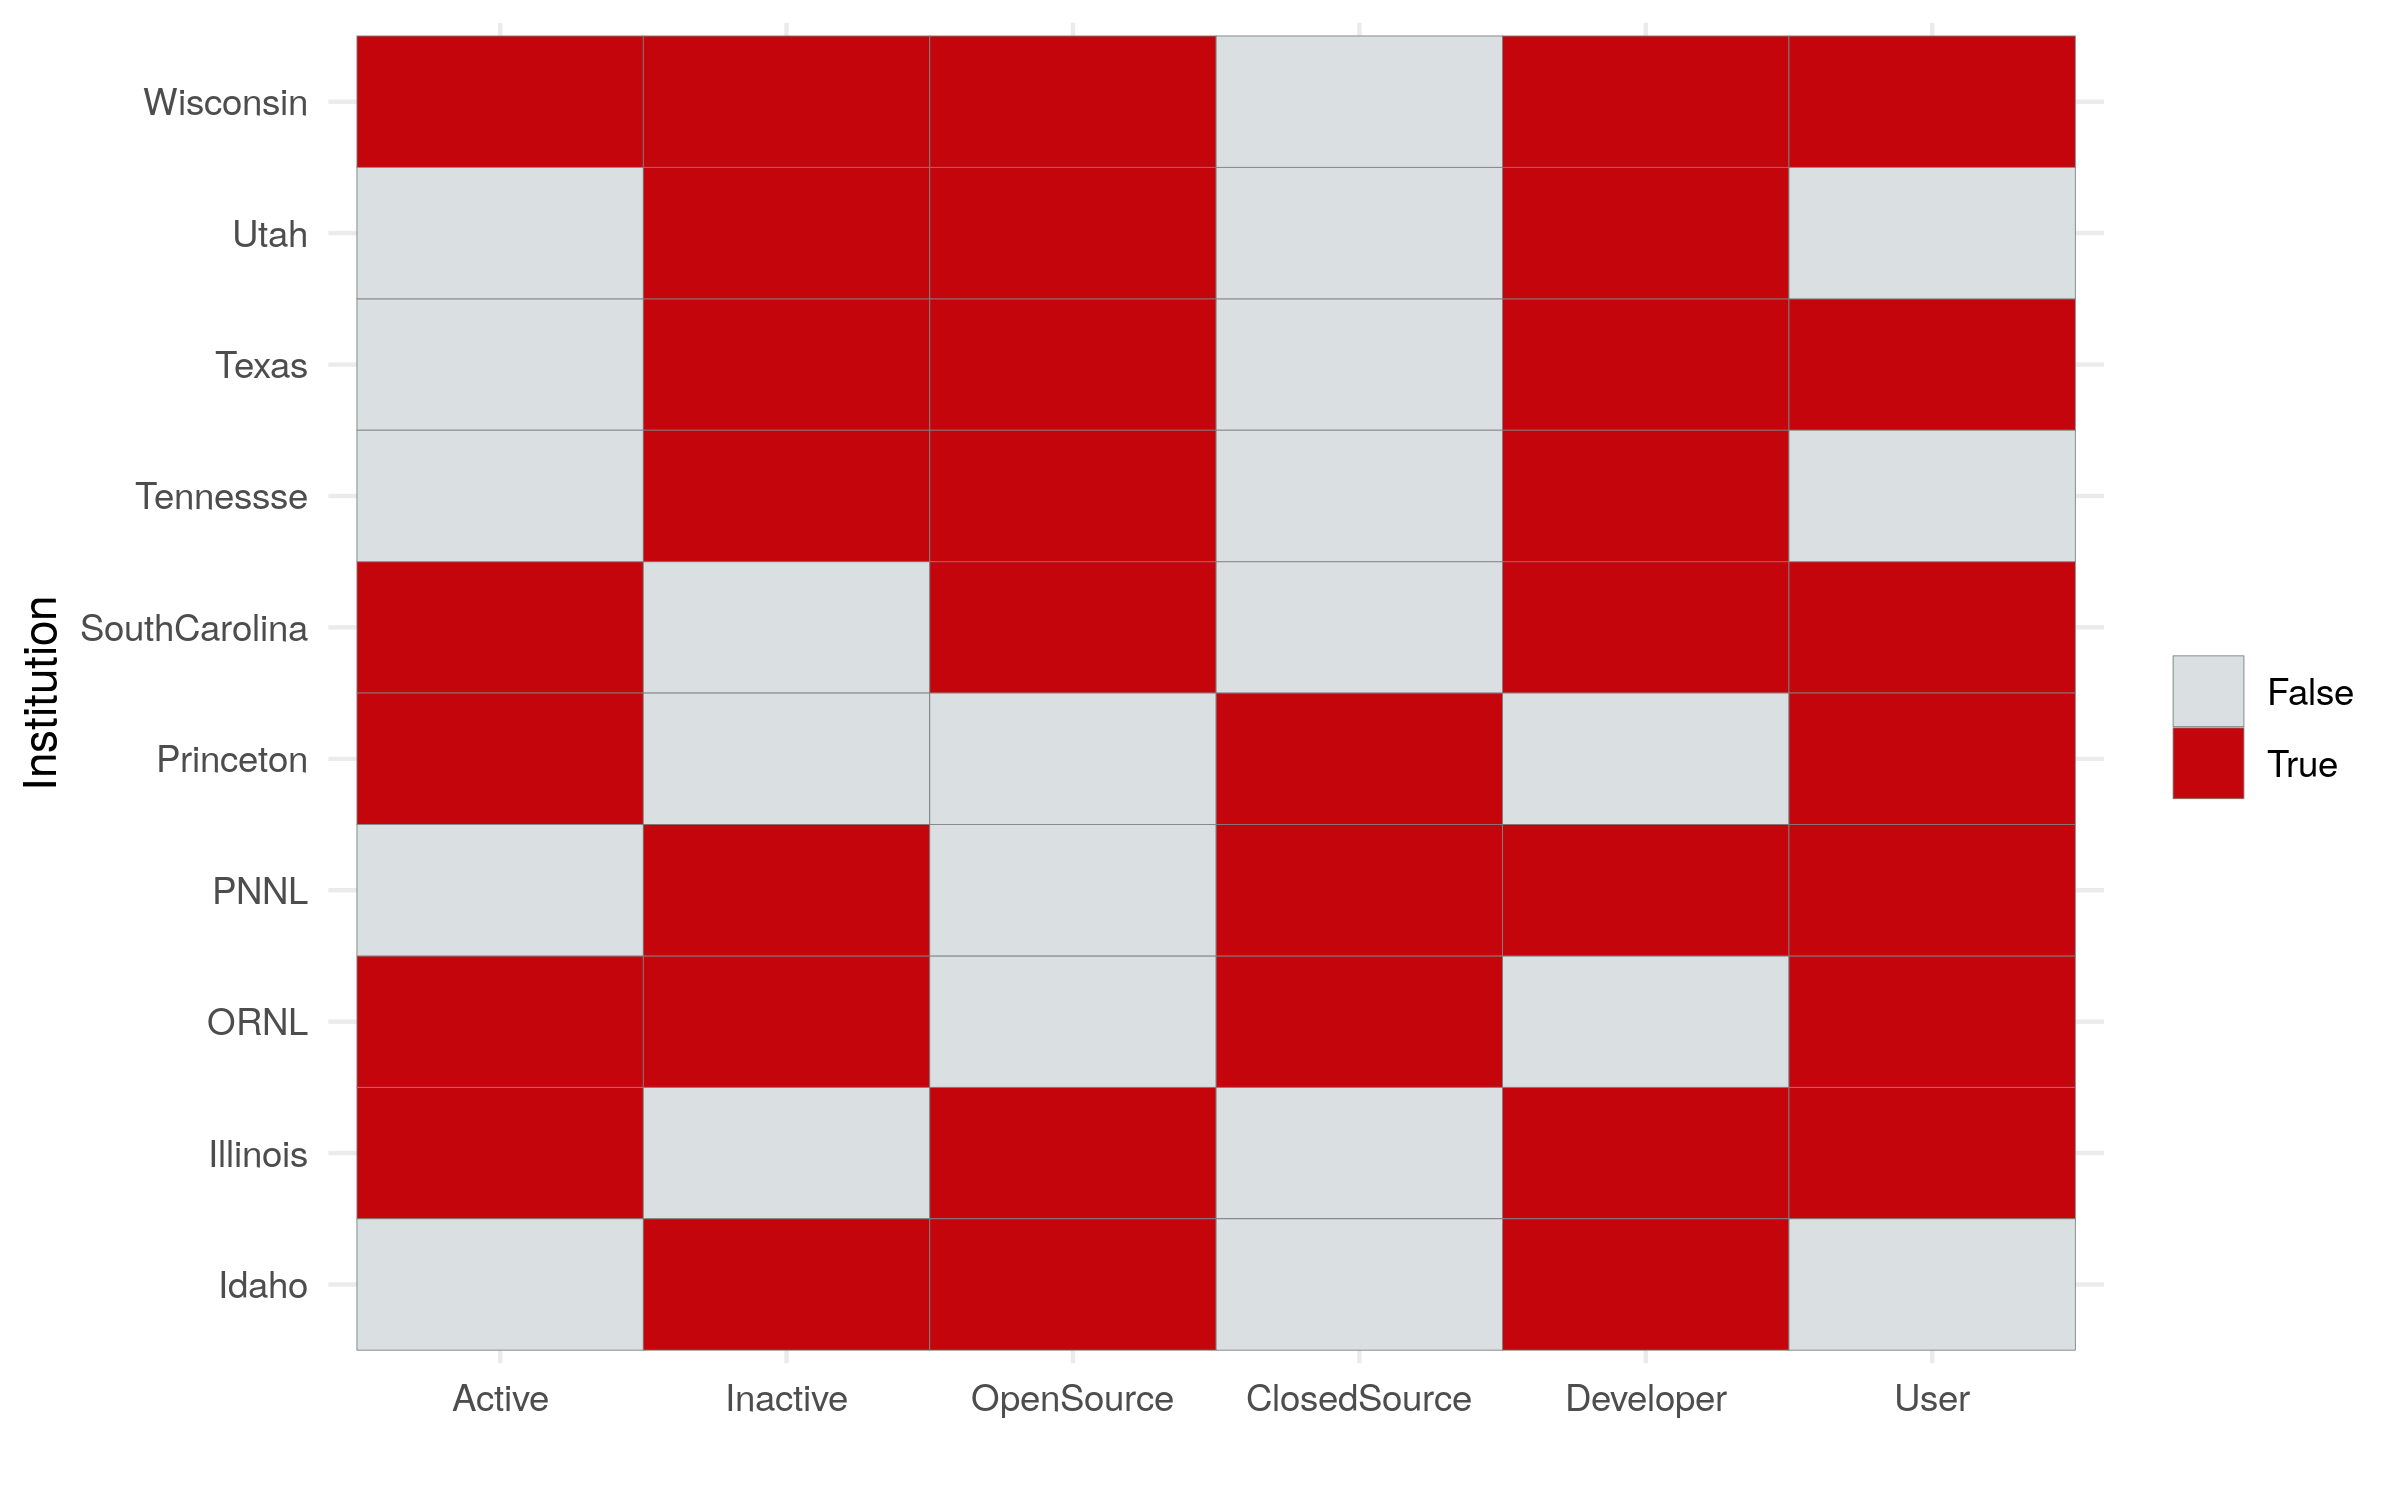
\includegraphics[width=\textwidth]{images/heat.png}
        \caption{Community is mainly university, national lab}
        \label{fig:my_label}
    \end{figure}
    \end{columns}
\end{frame}
% ---------------------------------------------- %

% ---------------------------------------------- %
\begin{frame}{\Cyclus Funders}
    \begin{columns}
    \column{0.6\textwidth}
    \begin{figure}
        \centering
        
\includegraphics[width=\textwidth]{images/Cyclus-funders.png}
        %\caption{}
        \label{fig:my_label}
    \end{figure}
    \column{0.3\textwidth}
    Diverse albeit intermittent funding sources over the last decade
    \end{columns}
\end{frame}
% ---------------------------------------------- %